% !TEX root = ../../main.tex

\section{Calorimetry dataset UiO-66(Zr)}

\begin{figure}[htb]
    \centering

    \begin{subfigure}{0.19\linewidth}
        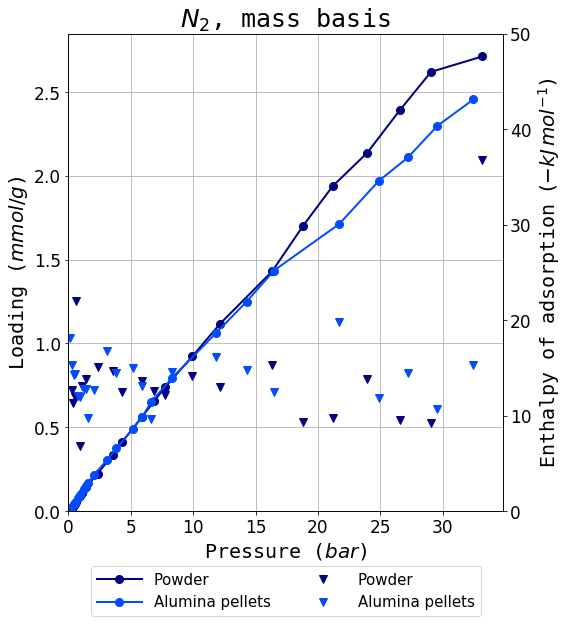
\includegraphics[width=\textwidth]{calo/UiO-66(Zr)/N2-mass-basis-iso}
        \label{fgr:uio66n2mass}
    \end{subfigure}
    \begin{subfigure}{0.19\linewidth}
        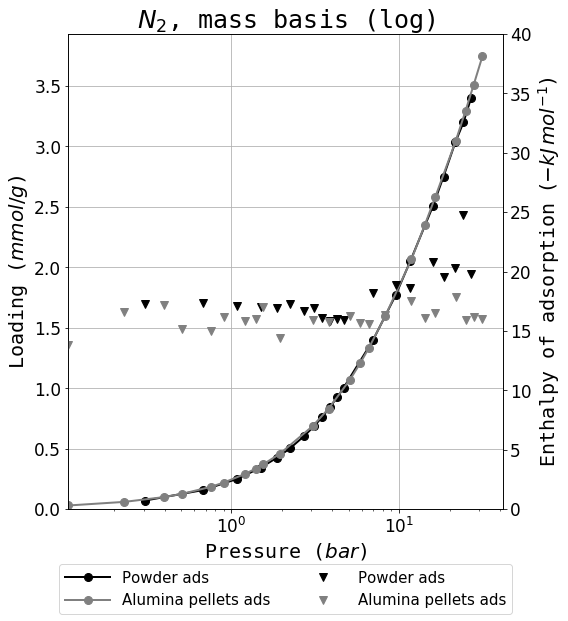
\includegraphics[width=\textwidth]{calo/UiO-66(Zr)/N2-mass-basis-log-iso}
        \label{fgr:uio66n2masslog}
    \end{subfigure}
    \begin{subfigure}{0.19\linewidth}
        \includegraphics[width=\textwidth]{calo/UiO-66(Zr)/{N2-volume-basis-iso}}
        \label{fgr:uio66n2volume}
    \end{subfigure}
    \begin{subfigure}{0.19\linewidth}
        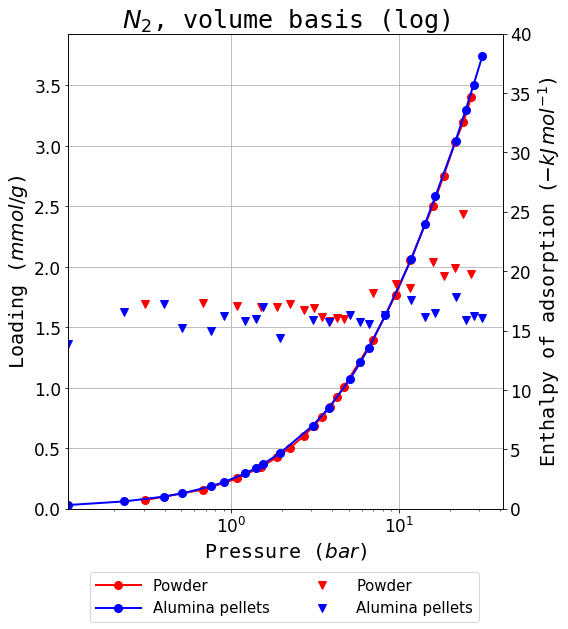
\includegraphics[width=\textwidth]{calo/UiO-66(Zr)/N2-volume-basis-log-iso}
        \label{fgr:uio66n2volumelog}
    \end{subfigure}
    \begin{subfigure}{0.19\linewidth}
        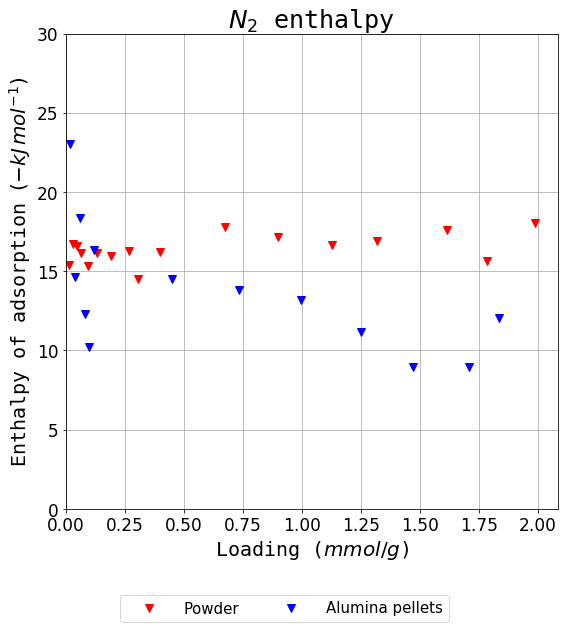
\includegraphics[width=\textwidth]{calo/UiO-66(Zr)/N2-enth}
        \label{fgr:uio66n2enth}
    \end{subfigure}
    

    \begin{subfigure}{0.19\textwidth}
        \includegraphics[width=\textwidth]{calo/UiO-66(Zr)/{co2-mass-basis-iso}}
        \label{fgr:uio66co2mass}
    \end{subfigure}
    \begin{subfigure}{0.19\textwidth}
        \includegraphics[width=\textwidth]{calo/UiO-66(Zr)/co2-mass-basis-log-iso}
        \label{fgr:uio66co2masslog}
    \end{subfigure}
    \begin{subfigure}{0.19\textwidth}
        \includegraphics[width=\textwidth]{calo/UiO-66(Zr)/{co2-volume-basis-iso}}
        \label{fgr:uio66co2volume}
    \end{subfigure}
    \begin{subfigure}{0.19\textwidth}
        \includegraphics[width=\textwidth]{calo/UiO-66(Zr)/co2-volume-basis-log-iso}
        \label{fgr:uio66co2volumelog}
    \end{subfigure}
    \begin{subfigure}{0.19\textwidth}
        \includegraphics[width=\textwidth]{calo/UiO-66(Zr)/co2-enth}
        \label{fgr:uio66co2enth}
    \end{subfigure}


    \begin{subfigure}{0.19\textwidth}
        \includegraphics[width=\textwidth]{calo/UiO-66(Zr)/{co-mass-basis-iso}}
        \label{fgr:uio66comass}
    \end{subfigure}
    \begin{subfigure}{0.19\textwidth}
        \includegraphics[width=\textwidth]{calo/UiO-66(Zr)/co-mass-basis-log-iso}
        \label{fgr:uio66comasslog}
    \end{subfigure}
    \begin{subfigure}{0.19\textwidth}
        \includegraphics[width=\textwidth]{calo/UiO-66(Zr)/{co-volume-basis-iso}}
        \label{fgr:uio66covolume}
    \end{subfigure}
    \begin{subfigure}{0.19\textwidth}
        \includegraphics[width=\textwidth]{calo/UiO-66(Zr)/co-volume-basis-log-iso}
        \label{fgr:uio66covolumelog}
    \end{subfigure}
    \begin{subfigure}{0.19\textwidth}
        \includegraphics[width=\textwidth]{calo/UiO-66(Zr)/co-enth}
        \label{fgr:uio66coenth}
    \end{subfigure}


    \begin{subfigure}{0.19\textwidth}
        \includegraphics[width=\textwidth]{calo/UiO-66(Zr)/{ch4-mass-basis-iso}}
        \label{fgr:uio66ch4mass}
    \end{subfigure}
    \begin{subfigure}{0.19\textwidth}
        \includegraphics[width=\textwidth]{calo/UiO-66(Zr)/ch4-mass-basis-log-iso}
        \label{fgr:uio66ch4masslog}
    \end{subfigure}
    \begin{subfigure}{0.19\textwidth}
        \includegraphics[width=\textwidth]{calo/UiO-66(Zr)/{ch4-volume-basis-iso}}
        \label{fgr:uio66ch4volume}
    \end{subfigure}
    \begin{subfigure}{0.19\textwidth}
        \includegraphics[width=\textwidth]{calo/UiO-66(Zr)/ch4-volume-basis-log-iso}
        \label{fgr:uio66ch4volumelog}
    \end{subfigure}
    \begin{subfigure}{0.19\textwidth}
        \includegraphics[width=\textwidth]{calo/UiO-66(Zr)/ch4-enth}
        \label{fgr:uio66ch4enth}
    \end{subfigure}

    \caption{Complete isotherm and enthalpy dataset for UiO-66(Zr)}
    
\end{figure}
\begin{figure}[htb]\ContinuedFloat%

    \begin{subfigure}{0.19\textwidth}
        \includegraphics[width=\textwidth]{calo/UiO-66(Zr)/{c2h6-mass-basis-iso}}
        \label{fgr:uio66c2h6mass}
    \end{subfigure}
    \begin{subfigure}{0.19\textwidth}
        \includegraphics[width=\textwidth]{calo/UiO-66(Zr)/c2h6-mass-basis-log-iso}
        \label{fgr:uio66c2h6masslog}
    \end{subfigure}
    \begin{subfigure}{0.19\textwidth}
        \includegraphics[width=\textwidth]{calo/UiO-66(Zr)/{c2h6-volume-basis-iso}}
        \label{fgr:uio66c2h6volume}
    \end{subfigure}
    \begin{subfigure}{0.19\textwidth}
        \includegraphics[width=\textwidth]{calo/UiO-66(Zr)/c2h6-volume-basis-log-iso}
        \label{fgr:uio66c2h6volumelog}
    \end{subfigure}
    \begin{subfigure}{0.19\textwidth}
        \includegraphics[width=\textwidth]{calo/UiO-66(Zr)/c2h6-enth}
        \label{fgr:uio66c2h6enth}
    \end{subfigure}


    \begin{subfigure}{0.19\textwidth}
        \includegraphics[width=\textwidth]{calo/UiO-66(Zr)/{c3h8-mass-basis-iso}}
        \label{fgr:uio66c3h8mass}
    \end{subfigure}
    \begin{subfigure}{0.19\textwidth}
        \includegraphics[width=\textwidth]{calo/UiO-66(Zr)/c3h8-mass-basis-log-iso}
        \label{fgr:uio66c3h8masslog}
    \end{subfigure}
    \begin{subfigure}{0.19\textwidth}
        \includegraphics[width=\textwidth]{calo/UiO-66(Zr)/{c3h8-volume-basis-iso}}
        \label{fgr:uio66c3h8volume}
    \end{subfigure}
    \begin{subfigure}{0.19\textwidth}
        \includegraphics[width=\textwidth]{calo/UiO-66(Zr)/c3h8-volume-basis-log-iso}
        \label{fgr:uio66c3h8volumelog}
    \end{subfigure}
    \begin{subfigure}{0.19\textwidth}
        \includegraphics[width=\textwidth]{calo/UiO-66(Zr)/c3h8-enth}
        \label{fgr:uio66c3h8enth}
    \end{subfigure}

    \begin{subfigure}{0.19\textwidth}
        \includegraphics[width=\textwidth]{calo/UiO-66(Zr)/{c3h6-mass-basis-iso}}
        \label{fgr:uio66c3h6mass}
    \end{subfigure}
    \begin{subfigure}{0.19\textwidth}
        \includegraphics[width=\textwidth]{calo/UiO-66(Zr)/c3h6-mass-basis-log-iso}
        \label{fgr:uio66c3h6masslog}
    \end{subfigure}
    \begin{subfigure}{0.19\textwidth}
        \includegraphics[width=\textwidth]{calo/UiO-66(Zr)/{c3h6-volume-basis-iso}}
        \label{fgr:uio66c3h6volume}
    \end{subfigure}
    \begin{subfigure}{0.19\textwidth}
        \includegraphics[width=\textwidth]{calo/UiO-66(Zr)/c3h6-volume-basis-log-iso}
        \label{fgr:uio66c3h6volumelog}
    \end{subfigure}
    \begin{subfigure}{0.19\textwidth}
        \includegraphics[width=\textwidth]{calo/UiO-66(Zr)/c3h6-enth}
        \label{fgr:uio66c3h6enth}
    \end{subfigure}


    \begin{subfigure}{0.19\textwidth}
        \includegraphics[width=\textwidth]{calo/UiO-66(Zr)/{c4h10-mass-basis-iso}}
        \label{fgr:uio66c4h10mass}
    \end{subfigure}
    \begin{subfigure}{0.19\textwidth}
        \includegraphics[width=\textwidth]{calo/UiO-66(Zr)/c4h10-mass-basis-log-iso}
        \label{fgr:uio66c4h10masslog}
    \end{subfigure}
    \begin{subfigure}{0.19\textwidth}
        \includegraphics[width=\textwidth]{calo/UiO-66(Zr)/{c4h10-volume-basis-iso}}
        \label{fgr:uio66c4h10volume}
    \end{subfigure}
    \begin{subfigure}{0.19\textwidth}
        \includegraphics[width=\textwidth]{calo/UiO-66(Zr)/c4h10-volume-basis-log-iso}
        \label{fgr:uio66c4h10volumelog}
    \end{subfigure}
    \begin{subfigure}{0.19\textwidth}
        \includegraphics[width=\textwidth]{calo/UiO-66(Zr)/c4h10-enth}
        \label{fgr:uio66c4h10enth}
    \end{subfigure}

    \caption{Complete isotherm and enthalpy dataset for UiO-66(Zr)}
    \label{fgr:calouio66}
\end{figure}
